\documentclass{article}
\usepackage[utf8]{inputenc}
\usepackage{amsmath}
\usepackage{amssymb}
\usepackage{amsfonts}
\usepackage{graphicx}
\usepackage{color}
\usepackage[]{algorithm2e}

\graphicspath{ {./graphics/} }

\numberwithin{equation}{section}
\setlength{\parindent}{0cm}

\title{Numerical Optimization and its Applications: Final Project}
\author{
    Shahaf Finder
    \and
    Roy Uziel
}
\date{July 2018}

\begin{document}

\maketitle

\section{Project Overview}
The goal of this project is to implement a simple neural network for classification of small dimention data.\\

The objective function will be softmax regression.\\
The network will have L residual layers (L is a parameter) of the shape:
\begin{equation*}
\begin{split}
 &  f(W_1, W_2, b, x) = x + W_2 \sigma (W_1 x + b)\\
 & W_1 \in \mathbb{R}^{n \times n}\\
 & W_2 \in \mathbb{R}^{n \times n}\\
 & b \in \mathbb{R}^{n}
\end{split}
\end{equation*}

\section{Objective Loss Function}
\begin{itemize}
 \item
  We've computed Softmax and Loss in \textbf{softmax.m} and \textbf{loss.m}.
  \item
  The derivatives for the Softmax are in \textbf{loss{\_}grad{\_}theta.m} (gradient by weights) and \textbf{loss{\_}grad{\_}x.m} (gradient by X).
  \item
  \textbf{test{\_}loss.m} is the gradient test for the loss function.
  \item
 \textbf{ loss{\_}SGD.m} is an SGD variant for the loss function.
  \item
  \textbf{Q3.m} is a script used to run the SGD.
\end{itemize}
We didn't notice a significant difference using different batch size and learning rate.\\

Results for learning rate: 0.005, batch size: 100\\

\begin{figure}[h!]
  \caption{Peaks Validation Data}
  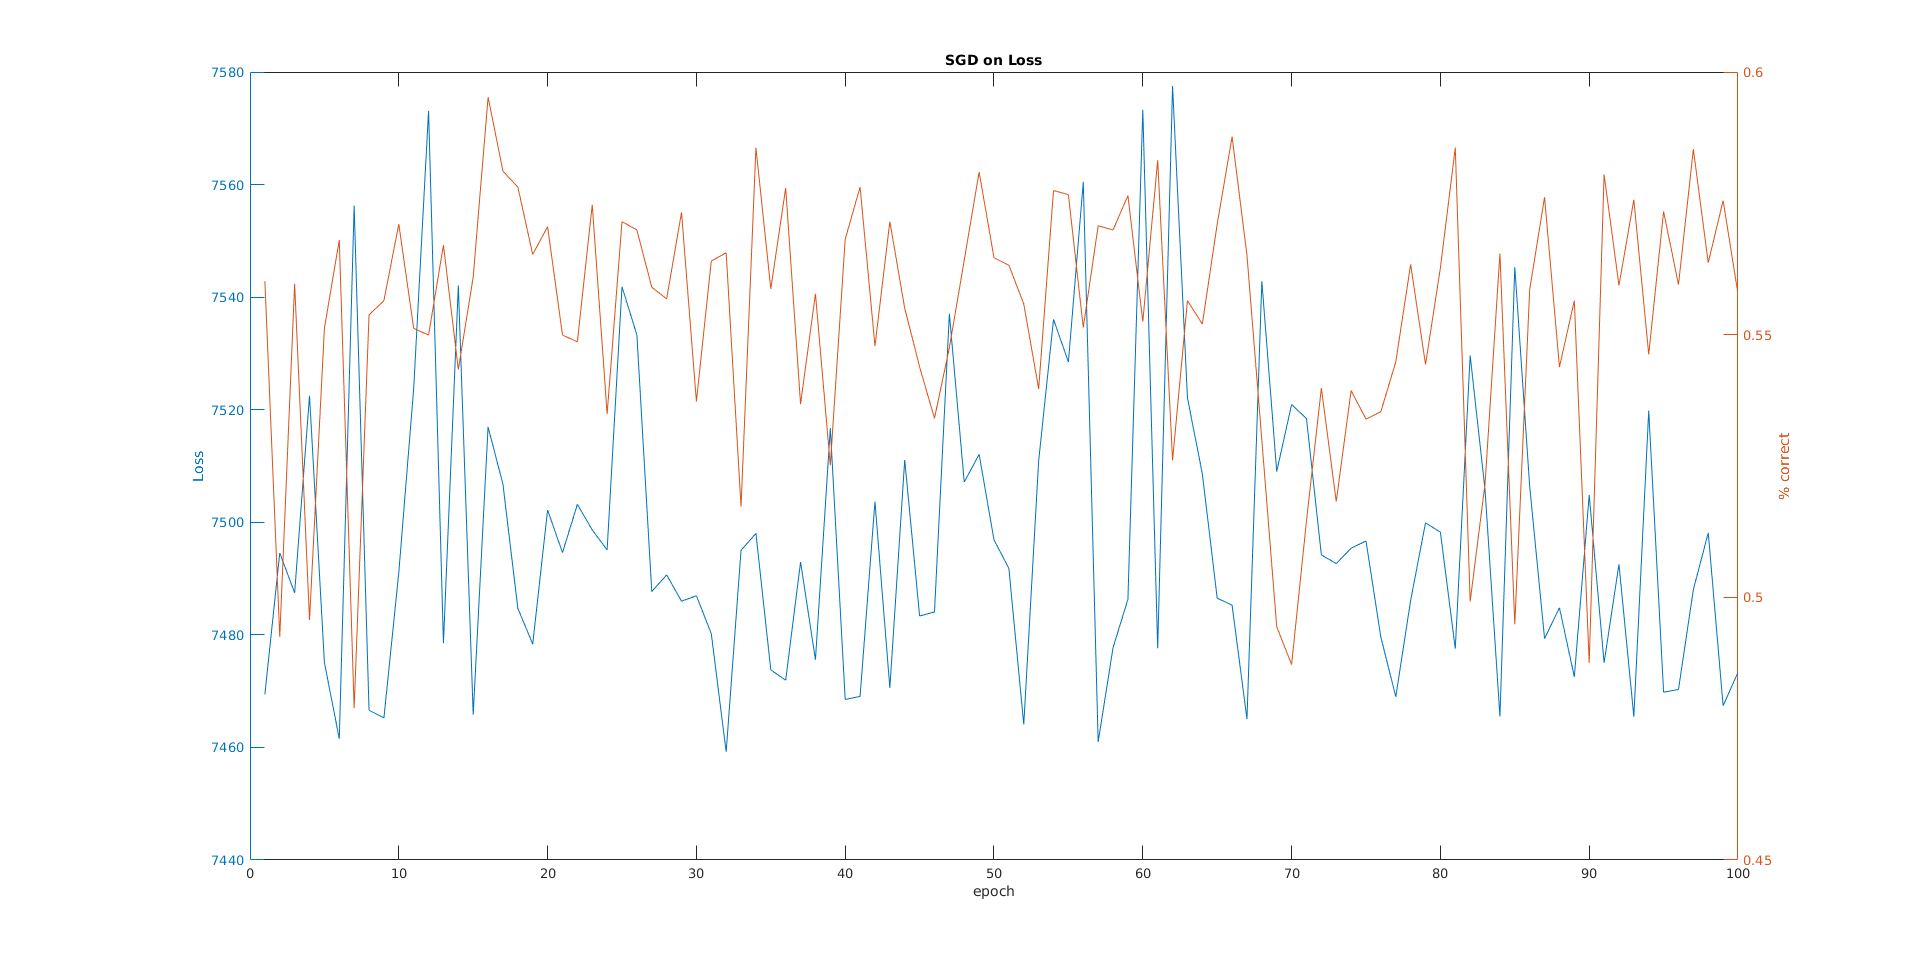
\includegraphics[width=\textwidth]{loss_sgd_val.png}
\end{figure}

\begin{figure}[h!]
  \caption{Peaks Training Data}
  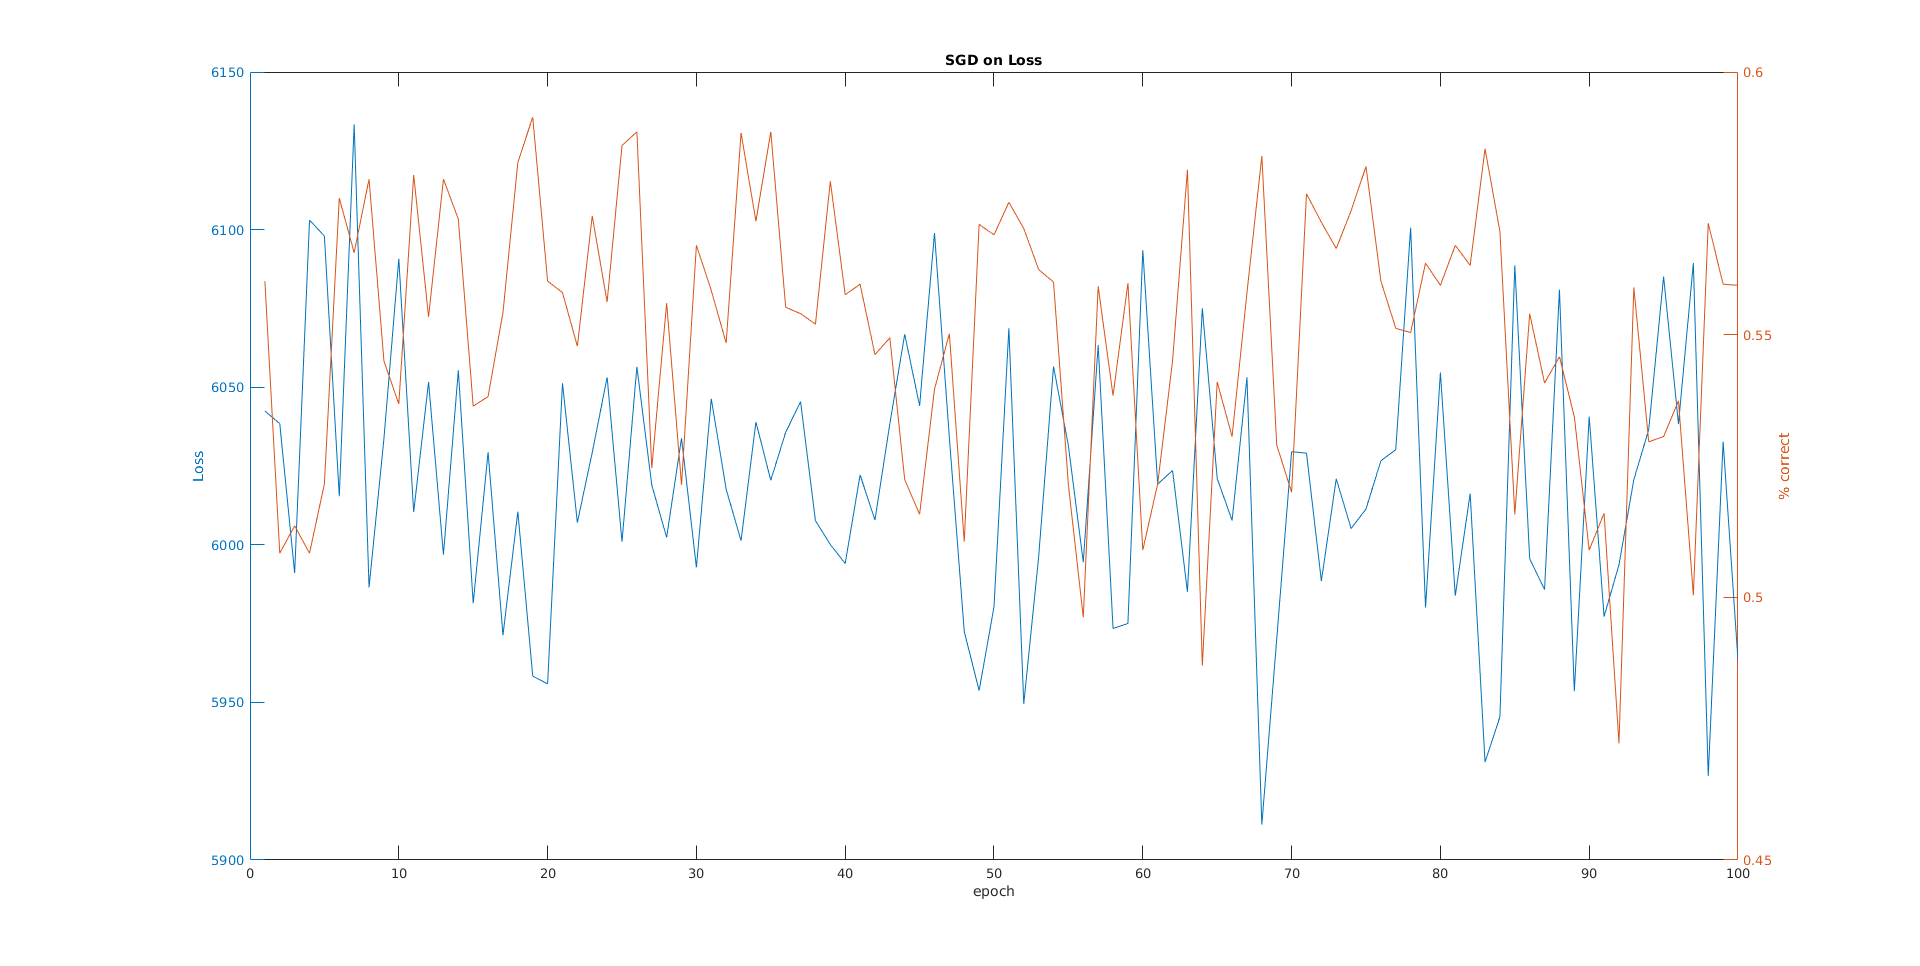
\includegraphics[width=\textwidth]{loss_sgd_train.png}
\end{figure}

\newpage

\section{Residual Neural Network}
\subsection{Jacobian Transpose Times Vector}
\textbf{ResNN{\_}jac{\_}theta{\_}t{\_}mul.m} and \textbf{ResNN{\_}jac{\_}x{\_}t{\_}mul.m} are the jacobian transpose times vector for each layer.\\

Both can receive multiple samples X (as an n times m matrix), and their respectives V (as an n times m matrix) to multiply by.
\begin{itemize}
\item 
\textbf{ResNN{\_}jac{\_}theta{\_}t{\_}mul.m} returns the average result among all samples.
\item
\textbf{ResNN{\_}jac{\_}x{\_}t{\_}mul.m} returns the multiplication of each sample with it's v (as an n times m matrix).
\end{itemize}

These functions are used in the back propagation process:\\
\begin{equation*}
\begin{split}
  & \nabla_{\theta^{(l)}}f_{l} = \frac{\delta f_{l}}{\delta \theta^{(l)}}^T \nabla_{x^{(l+1)}}f_{l+1}\\
  & \nabla_{x^{(l)}}f_{l} = \frac{\delta f_{l}}{\delta x^{(l)}}^T \nabla_{x^{(l+1)}}f_{l+1}
\end{split}
\end{equation*}

In order to test those functions we've created two auxiliary functions ResNN{\_}jac{\_}theta{\_}mul.m ResNN{\_}jac{\_}x{\_}mul.m\\
These auxiliary functions compute:
\begin{equation*}
  \frac{\delta f}{\delta \theta} v, 
  \frac{\delta f}{\delta x} v
\end{equation*}

We used the gradient test to make sure these functions are correct, and then used the jacobian transpose test with the required functions.\\
Those tests are in \textbf{test{\_}resnn.m}.

\subsection{Forward Pass and Back Propogation}
\textbf{forward{\_}pass.m} and \textbf{back{\_}propogation.m} are the implementations.\\

To test them we created test{\_}net.m that uses forward pass and back propogation to compute the gradient,\\
then each iteration we used forward pass to compute the loss value after moving to a direction.\\

\subsection{SGD and Conclusions}
\textbf{ResNN{\_}SGD.m} is the SGD variant for the entire network.\\
\textbf{run{\_}net.m} is a script used to run the SGD.\\

We've tested different network lengths and batch sizes on different data sets.\\
We got to the following conclusions:\\
\begin{itemize}
  \item
  Increasing batch size increased the training time, and above 50 it had little effect on results.
  \item
  Each dataset required different network lengths for good results.
  \item
  Lowering the learning rate resulted in a more steady but slower convergence. We found out that, generally, 0.01 is a good balance between speed and steadiness.
\end{itemize}

\begin{figure}[h!]
  \caption{GMM validation Data - 3 layer}
  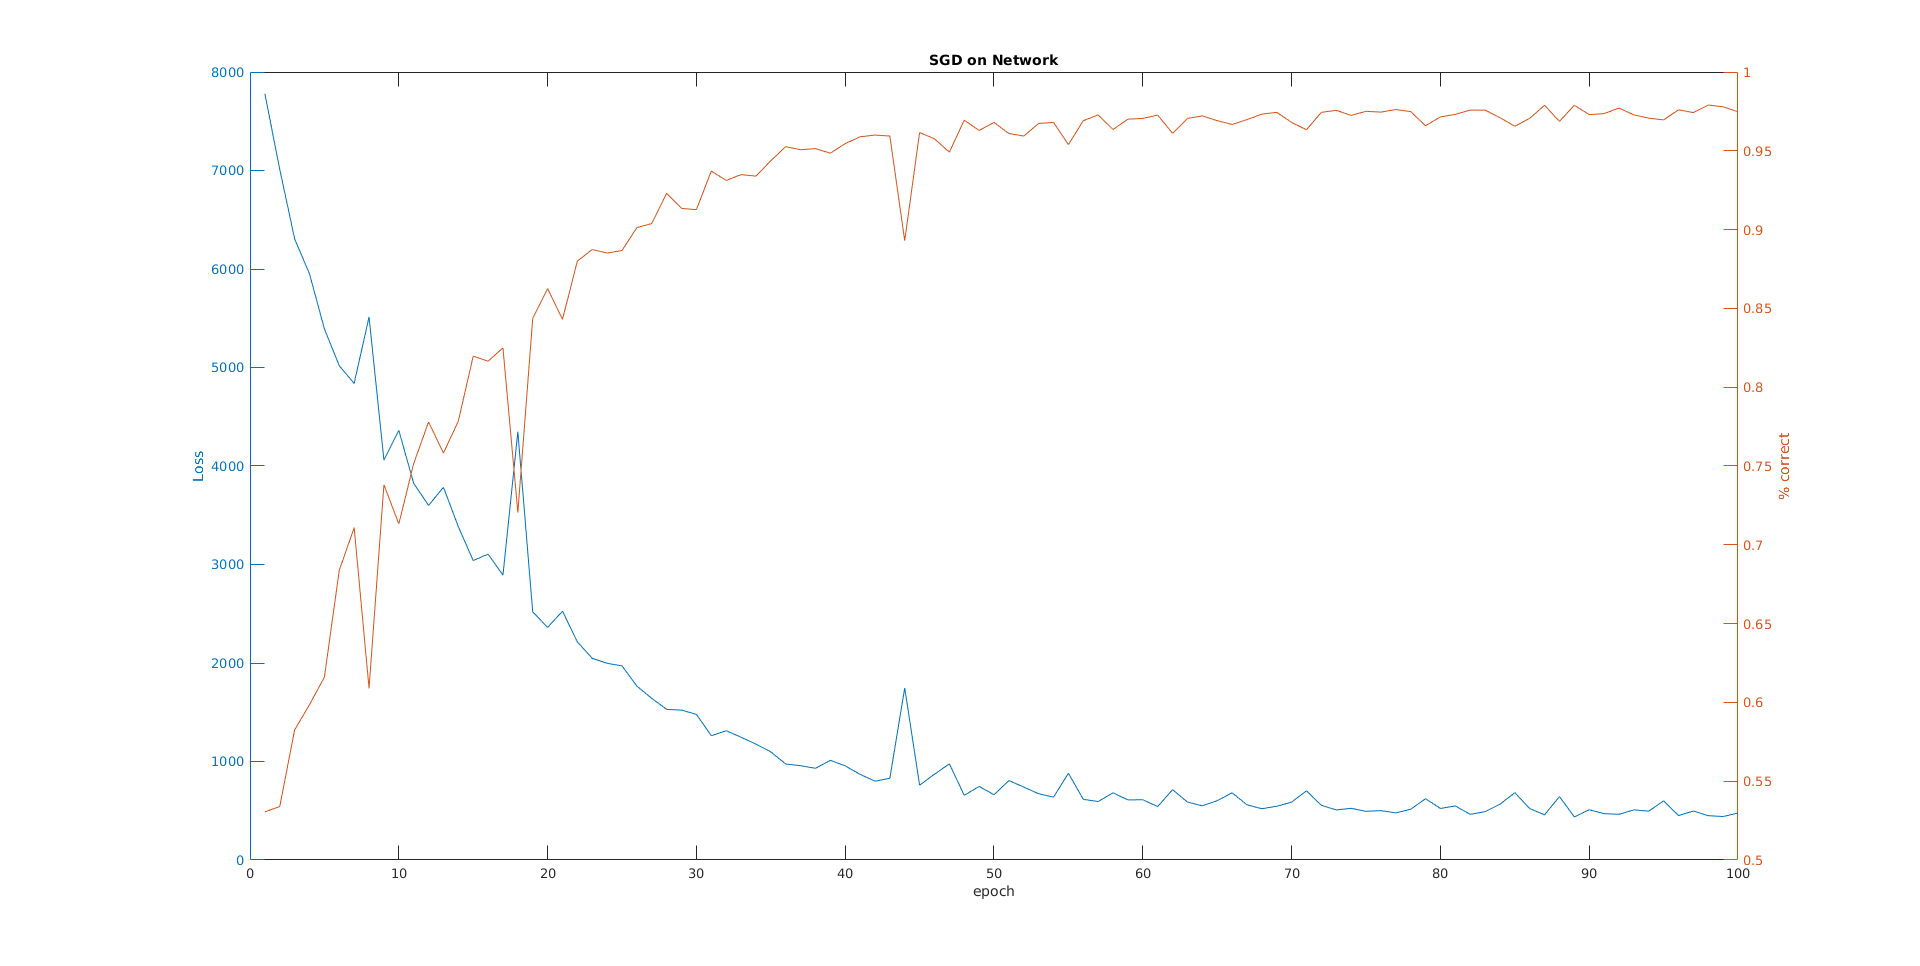
\includegraphics[width=\textwidth]{network_gmm_3layers.png}
\end{figure}

\begin{figure}[h!]
  \caption{Peaks validation Data - 10 layer}
  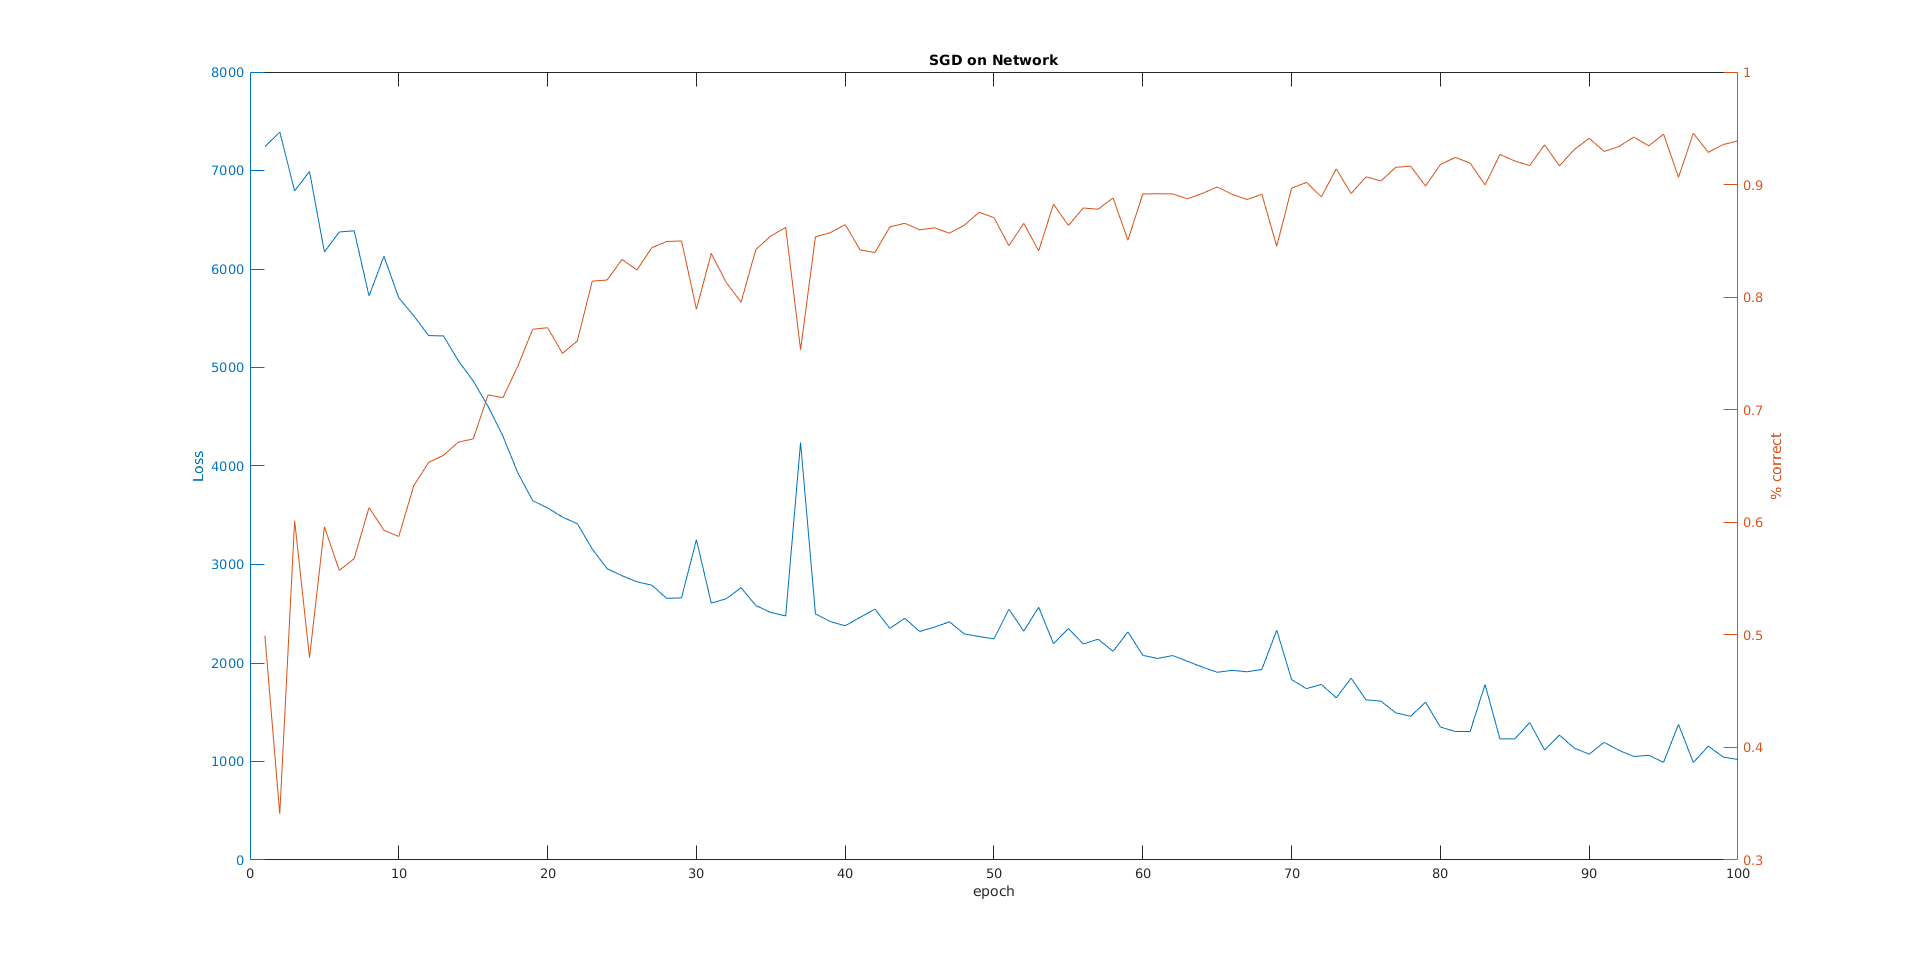
\includegraphics[width=\textwidth]{network_peaks_10layers.png}
\end{figure}

\begin{figure}[h!]
  \caption{SwissRoll validation Data - 15 layer}
  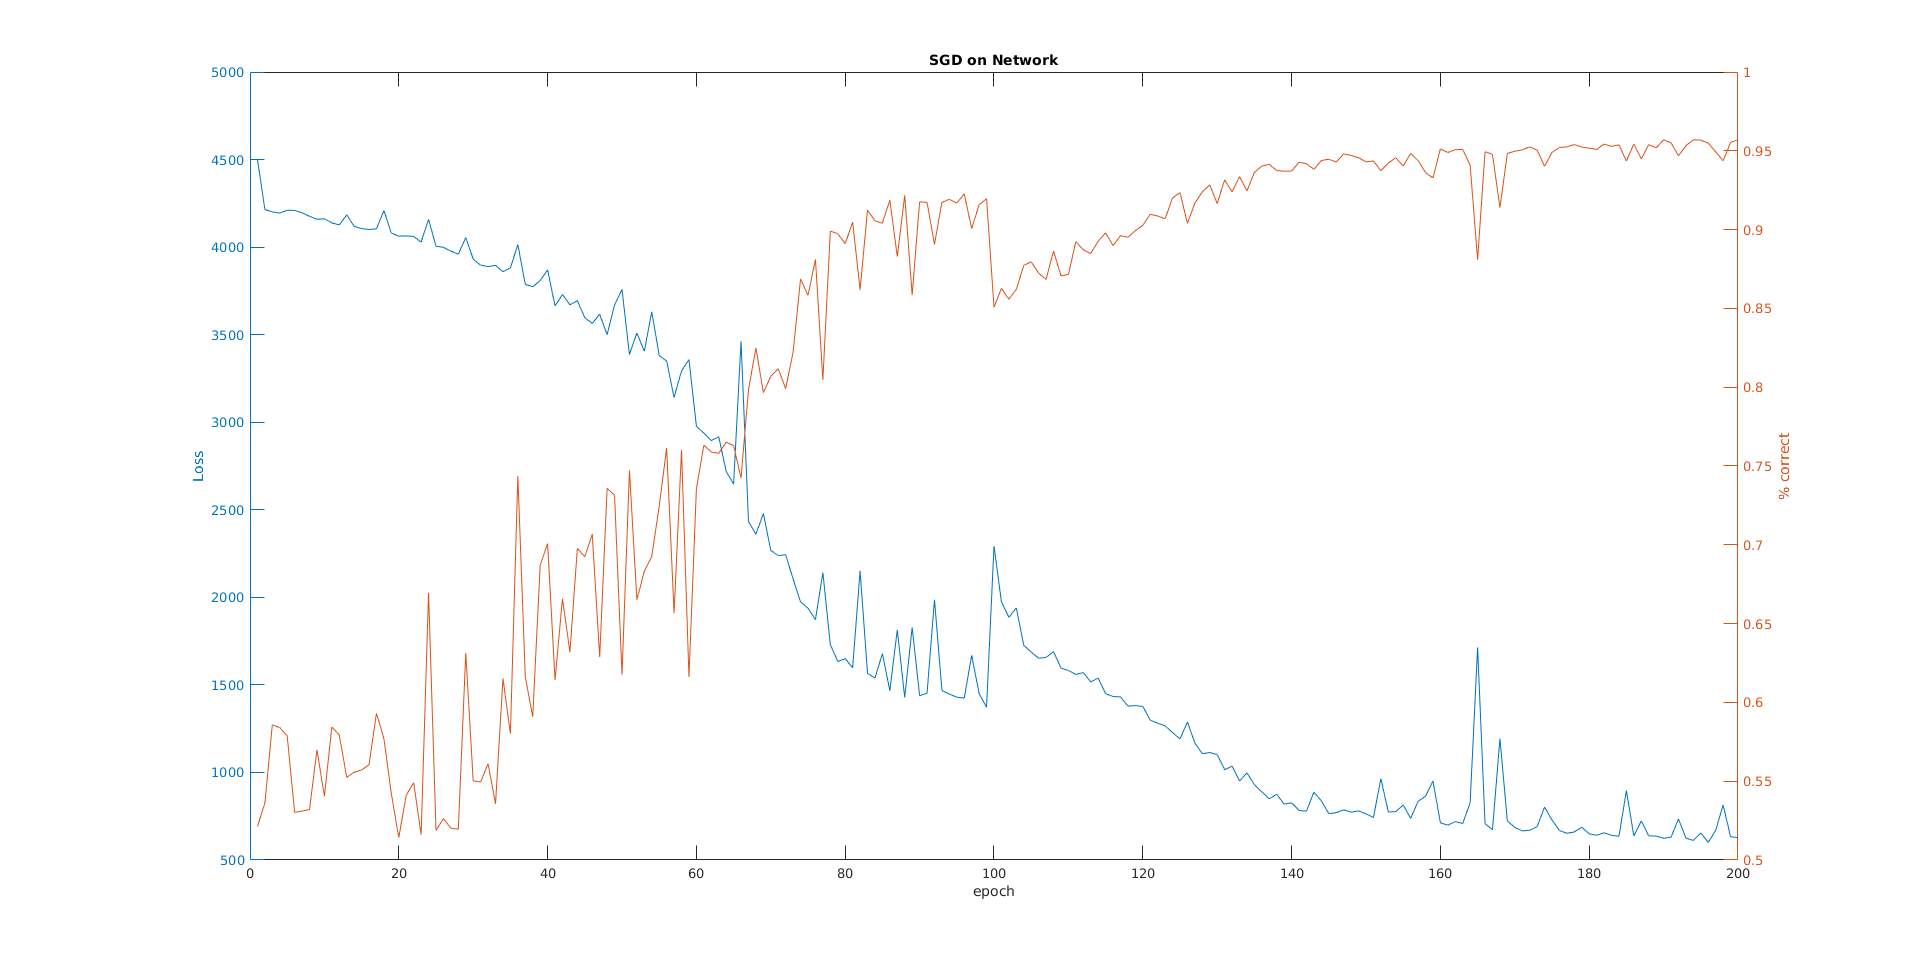
\includegraphics[width=\textwidth]{network_swissroll_15layers.png}
\end{figure}

\newpage

\section{Improving on SGD}
In seek to improve the results of SGD, we tried the following:
\begin{itemize}
 \item 
 Decreasing alpha according to iteration\\
 After 100 iterations we calculated a new alpha by: $learning{\_}rate * 5 / sqrt(i)$.\\
 This is in order to half the learning rate and keep decreasing as the iterations continue.\\
 The method gave minor improvement.
 \item
 Adding momentum (as seen in class)\\
 The method got much better results in convergence speed, but was unsteady in the long run.\\
 So in order to deal with the unsteadiness, after 100 iterations we calculated a new gamma using: $moment{\_}gamma * 10 / sqrt(i)$.\\
 This decreases the momentum as itereations continue.\\
 The results were a fast convergence in a more steady way.
 \item
 Taking only the rejection part of the momentum.\\
 While trying to optimize even further, we tried to take only the projection of the momentum over the gradient.\\
 We calculated it by: $m{\_}proj = g * m' * g / (norm(g)^2)$.\\
 We found out that by adding only the projection part, the results got worse, so we tried adding the rejection part.\\
 Calculated by: $m{\_}rej = m - m{\_}proj$.\\
 The results were usually better, or at worse - the same, than the normal momentum.
\end{itemize}

Using these 3 imrovements made us able to reduce the number of layers without hurting the results too much.

\newpage

Comparison between the 3 improvements.\\

All of the following figures are with the following parameters - batch size: 50, learning rate: 0.01, gamma (only for momentum): 0.7\\
Each figure shows 3 different run with each of the 3 improvements, made with the same initial weights (chosen randomly) and same seed for randperm (chosen randomly).\\

Blue - Using decreasing alpha only.\\
Orange - Using decreasing alpha, and decreasing momentum.\\
Yellow - Using all of the improvements specified above.\\

\begin{figure}[h!]
  \caption{GMM Data - 1 layer}
  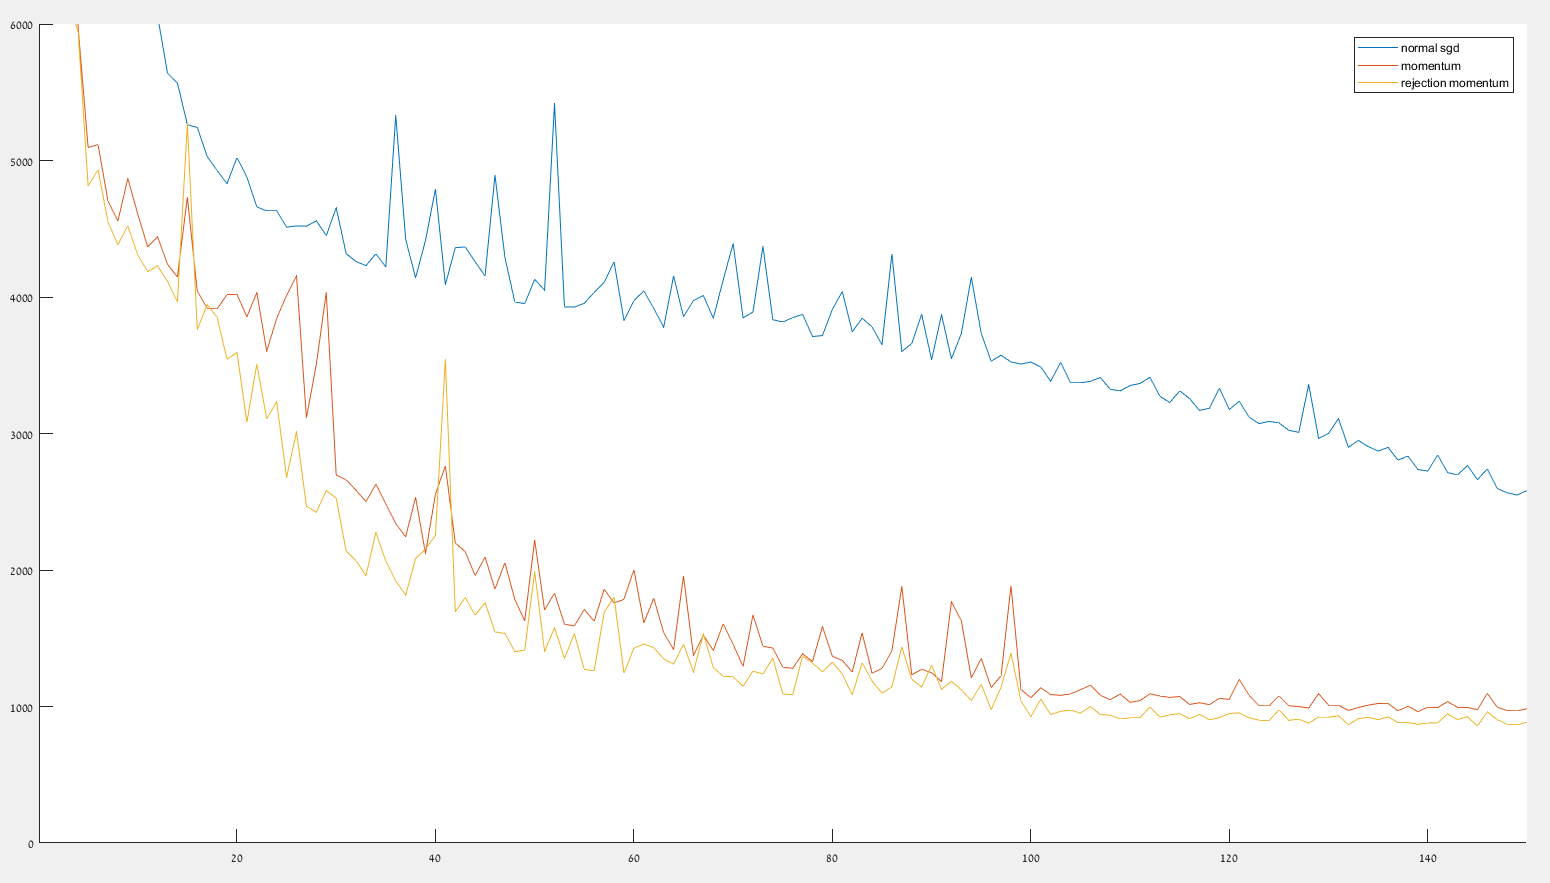
\includegraphics[width=\textwidth]{rej_m_gmm_1layer.png}
\end{figure}

\begin{figure}[h!]
  \caption{GMM Data - 2 layer}
  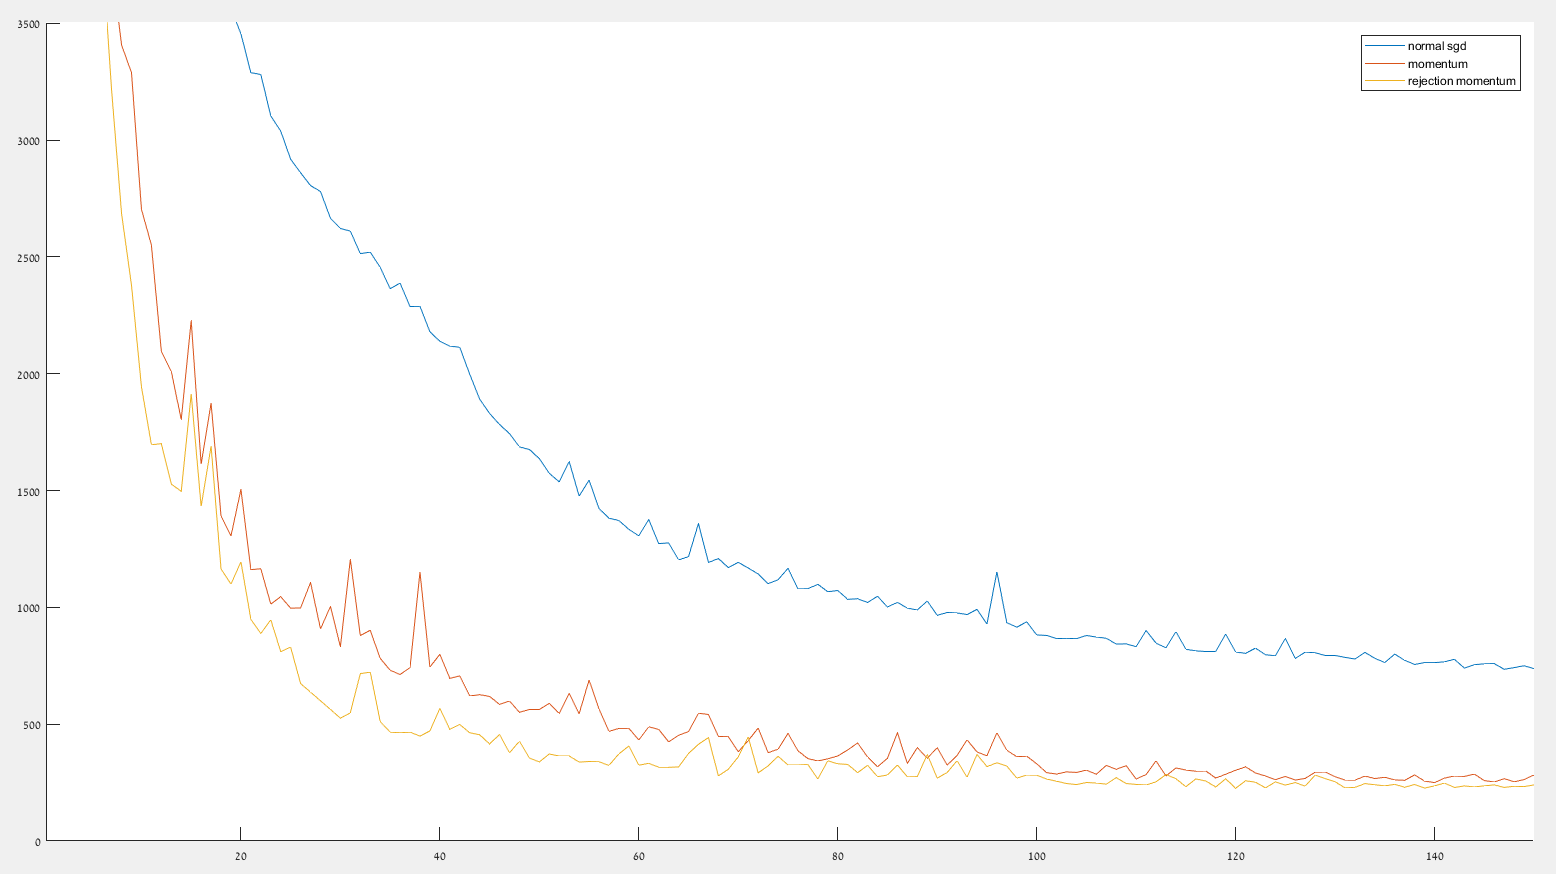
\includegraphics[width=\textwidth]{rej_m_gmm_2layers.png}
\end{figure}

\begin{figure}[h!]
  \caption{Peaks Data - 4 layer}
  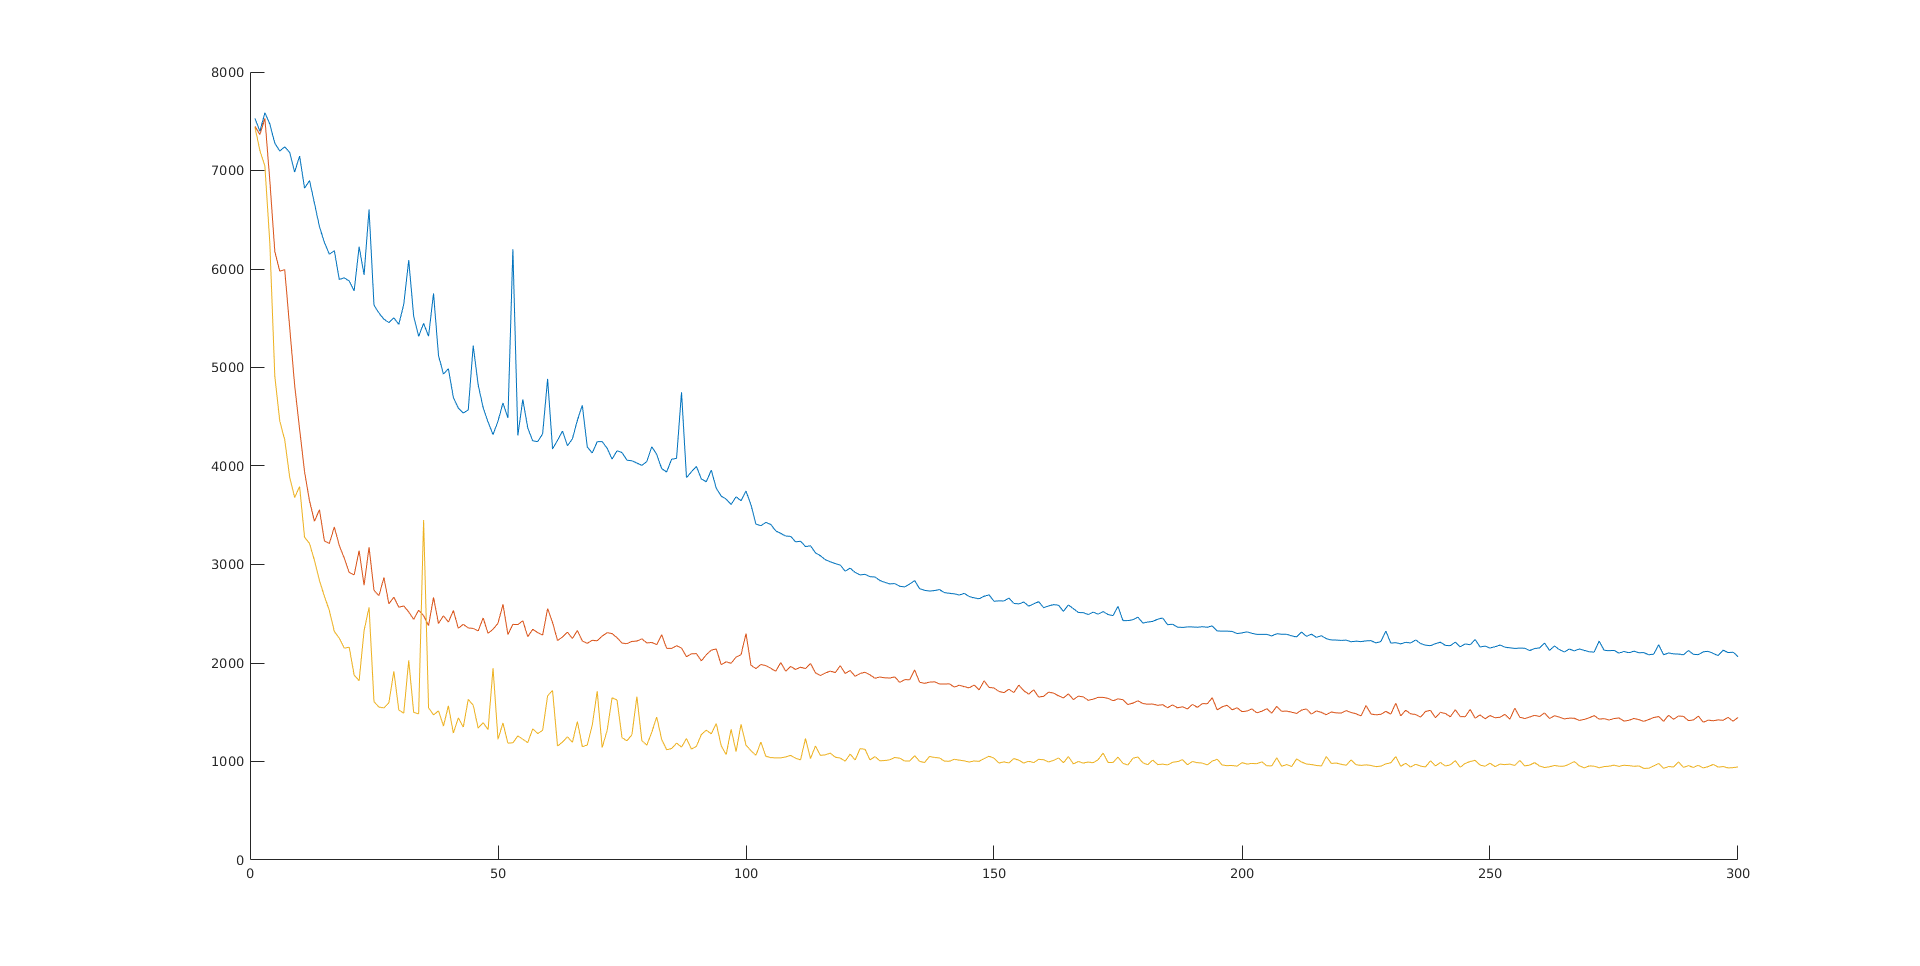
\includegraphics[width=\textwidth]{rej_m_peaks_4layers.png}
\end{figure}

\begin{figure}[h!]
  \caption{Peaks Data - 6 layer}
  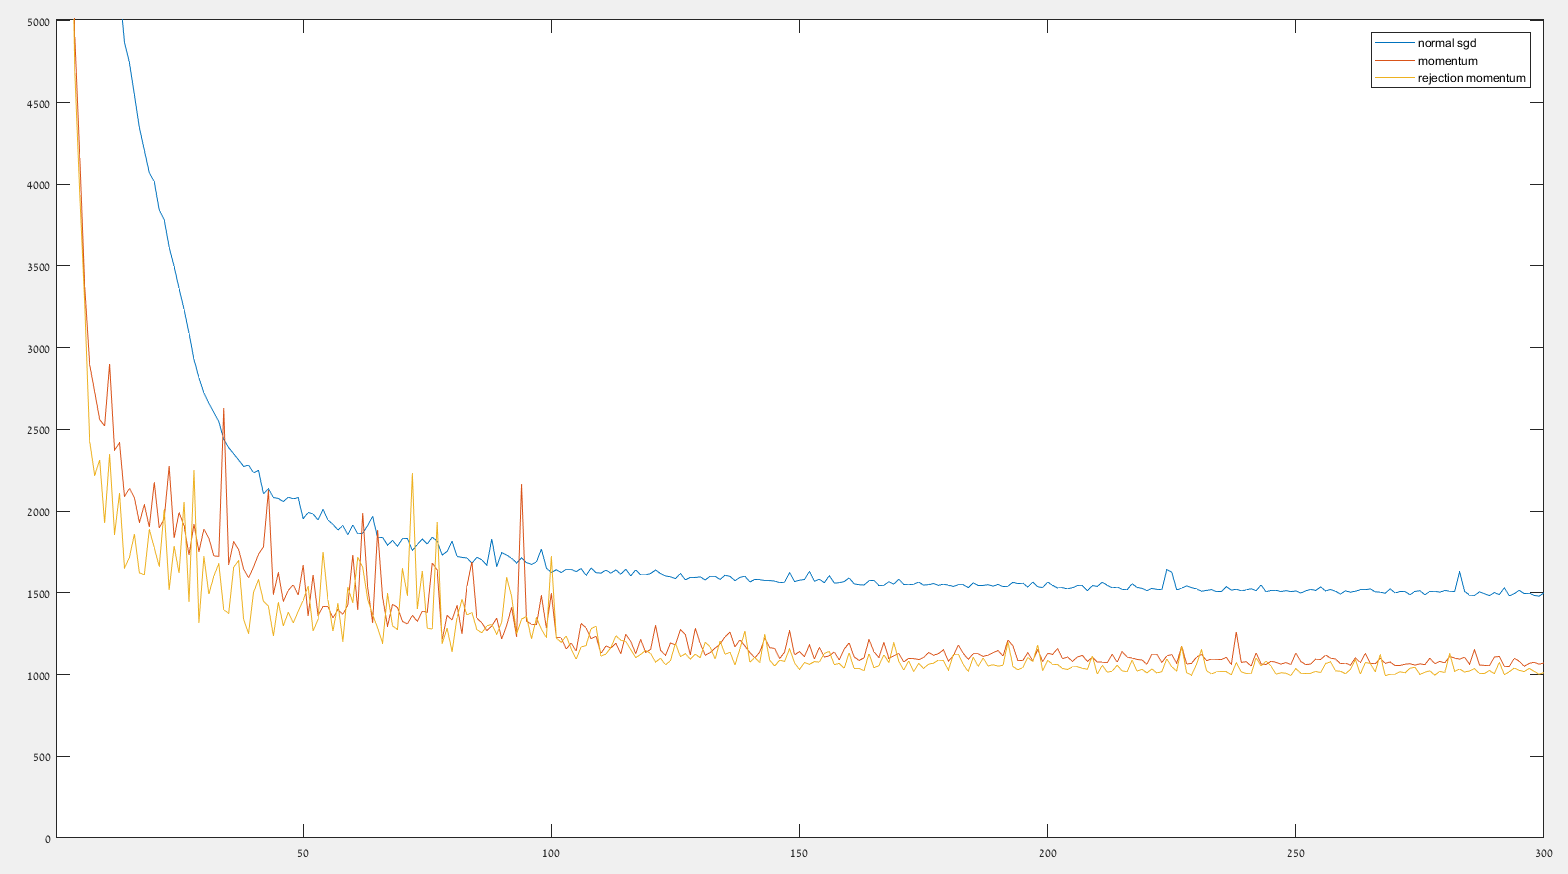
\includegraphics[width=\textwidth]{rej_m_peaks_6layers.png}
\end{figure}

\begin{figure}[h!]
  \caption{SwissRoll Data - 4 layer}
  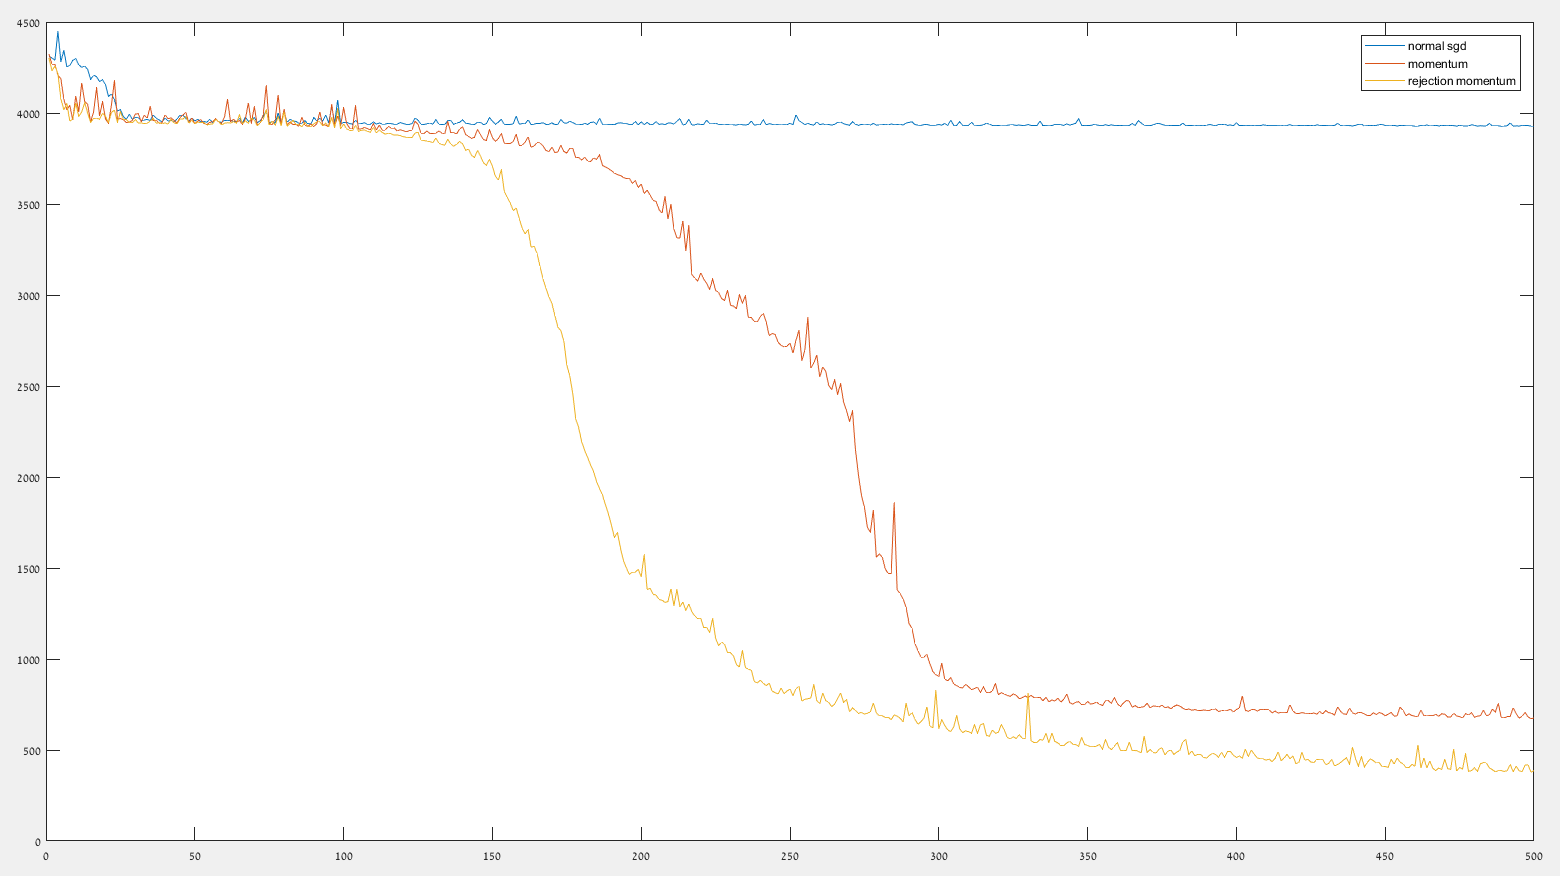
\includegraphics[width=\textwidth]{rej_m_swissroll_4layers.png}
\end{figure}

\begin{figure}[h!]
  \caption{SwissRoll Data - 5 layer}
  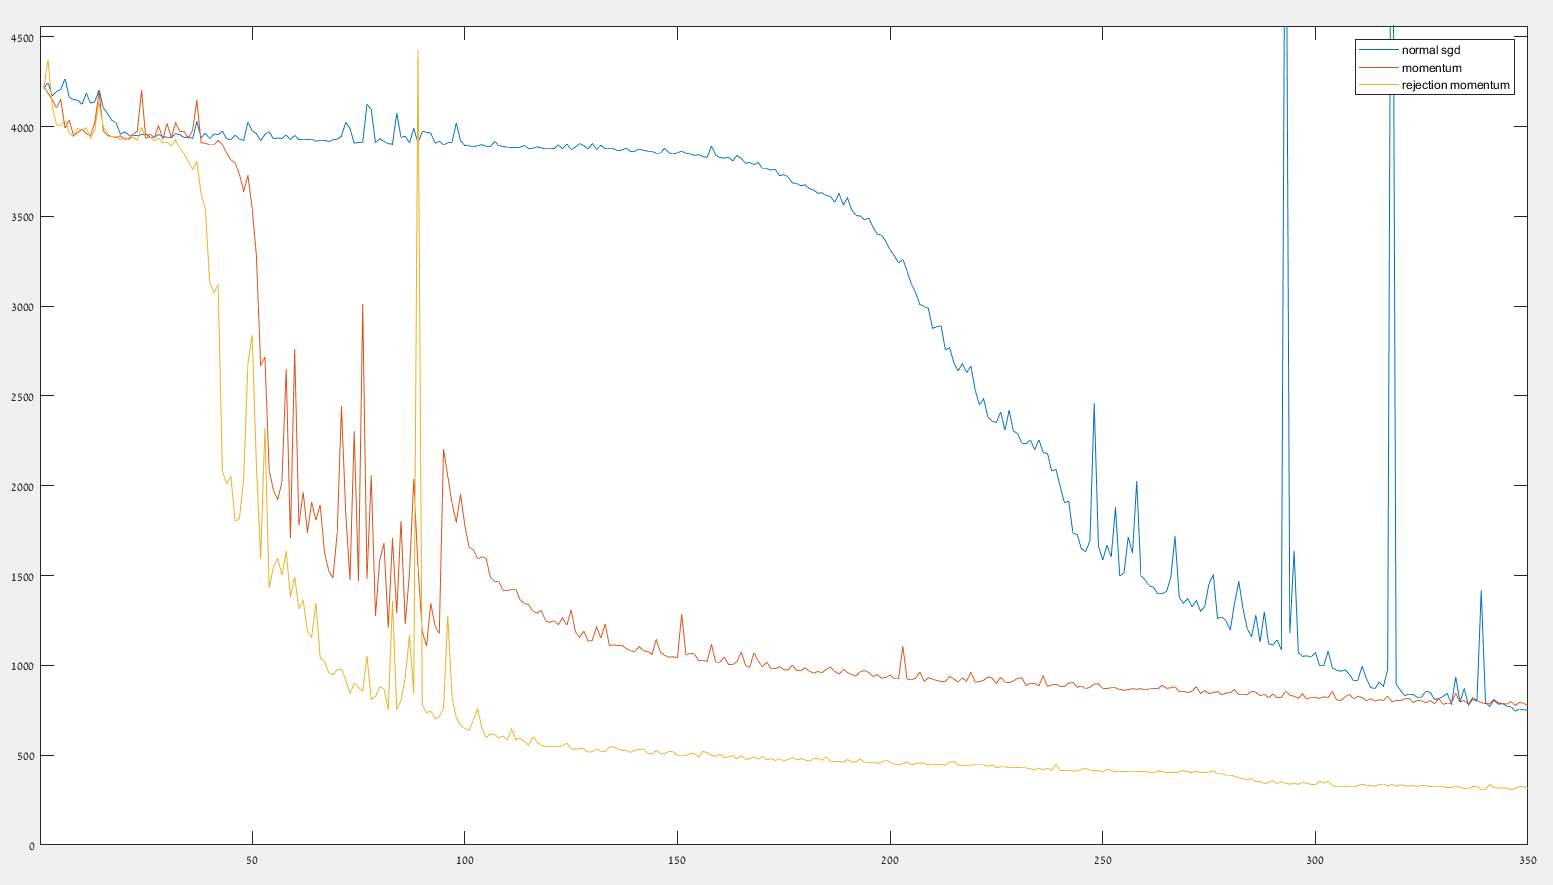
\includegraphics[width=\textwidth]{rej_m_swissroll_5layers.png}
\end{figure}

\end{document}
